\documentclass[a4paper,11pt]{report}
\usepackage[utf8]{inputenc}
\usepackage{geometry, amsmath, amsthm, latexsym, amssymb, graphicx}
\usepackage{amsmath,algorithm,algpseudocode}
\usepackage{hyperref}
\usepackage{gensymb}

\usepackage{environ}
\usepackage{tabto,enumitem}
\usepackage{lipsum}
\usepackage{makeidx}
\usepackage{blindtext}
\usepackage{enumitem}

\title{The arccosine function}
\author{Himansi Patel - 40072262}

\begin{document}
\begin{titlepage}
	\centering 
	
	\vspace*{4\baselineskip} 
	
	\rule{\textwidth}{1.6pt}\vspace*{-\baselineskip}\vspace*{2pt} 
	\rule{\textwidth}{0.4pt} 
	
	\vspace{0.75\baselineskip} 
	
	{\scshape \LARGE SOEN 6011 - Software Engineering Processes\\}
	
	{\scshape \LARGE Deliverable 2\\} 
	
	\vspace{0.75\baselineskip}
	
	\rule{\textwidth}{0.4pt}\vspace*{-\baselineskip}\vspace{3.2pt} 
	\rule{\textwidth}{1.6pt}
	
	\vspace{2\baselineskip} 
	
	\vspace*{3\baselineskip} 

	{\Large Submitted to\\ } 
	
	\vspace{0.2\baselineskip} 
	
	{\Large Prof. Pankaj Kamthan \\} 
	
	
	\vspace*{3\baselineskip} 
	
	{\Large By\\ } 
	\vspace{0.2\baselineskip} 
	
	{\Large Himansi Patel (40072262)\\ } 
	{\large Github id : https://github.com/Himansipatel/SOEN-6011-Team-H-Himansi \\}
	


\end{titlepage}
\newpage
\tableofcontents
\newpage

\section{Problem 4}
\subsection{Function Implementation}
The arccosine of x is defined as the inverse cosine function of x when -1$\leq$x$\leq$1.
It is most useful when trying to find the angle measure when two sides of a triangle are known.
There are various possible approaches to solve arccosine function using Taylor's
Series with recursive and iterative manner.I have implemented arccosine function using Taylor's
Series in iterative manner for its evaluation seemed most appropriate.\\
In general,
\begin{equation}
    \arccos x = \frac{\pi}{2}-\sum_{n=0}^\infty\frac{(2n)!}{2^{2n}(n!)^{2}}\frac{x^{2n+1}}{(2n+1)},|x|\textless1\\
\end{equation}


\begin{figure}[h]
    \centering
    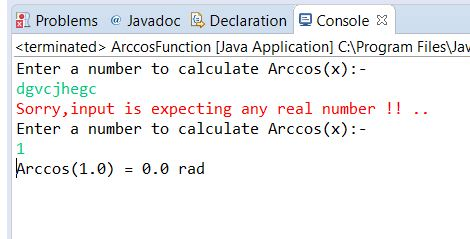
\includegraphics[width=0.99\textwidth]{guii.JPG}
    \caption{Graphical User Interface of implementation}
    \label{fig:guii}
\end{figure}

\newpage
\subsection{Eclipse Debugger}


\begin{itemize}
 \item\textbf{Introduction : }Debugging is a technical procedure used to detect and diagnose bugs in our program running either locally or remotely and eliminate them within a program in an effective way. Java debugger is a command line utility which allows in debugging developed java codes with real time values. We can review the constraints which we are using in our program with eclipse debugger.\\
 \item \textbf{Advantages : }
 \begin{enumerate}
     \item The debugger permits us to control the execution of our program by setting breakpoints, suspending launched programs, stepping through our code, and examining the contents of variables.\\
     \item The Eclipse platform has an advanced debugging feature which can be very beneficial in examination of our code through execution.\\
     \item In Eclipse, we can use the same platform for both development and debugging.\\
     \item ‘Debug Perspective’ is one of the valuable features of Eclipse which displays relevant debugging information side by side, such as variables, breakpoints, threads, and call stacks.\\
     \item The debugger has a client/server design so that we can debug programs running remotely on other systems in the network as well as programs running locally on our workstation.
     
 \end{enumerate}
 \item \textbf{Disadvantages : }
 \begin{enumerate}
     \item To evaluate some expressions to see its value, we need to select whole expression in eclipse otherwise eclipse cannot evaluate it. With IDEA, we don’t need to select anything. We just need to put cursor at any place inside the expression and press Alt+F8. It automatically understands which expression you probably need which makes it easier and faster.
 \end{enumerate}
 \end{itemize}
 
 \newpage
 \subsection{Quality Attributes}
 \begin{itemize}
 \item \textbf{Correct : }My application for the arccosine function is calculating the accurate result of the function. It gives exact results up to 2 decimal points. It is free from any error and it fulfills all the requirements of the function. I have tested correctness of my function by using different test cases.\\
 \item \textbf{Efficient : }My application generates results in stipulated time. It utilizes disk space and memory in  an efficient manner. It releases used resources as soon as the task is done so they can be utilized again. Also, it is not using all the available resources which makes it efficient so that it can be used in real time applications.\\
 \item \textbf{Maintainability : }It is very easy to add code to existing system and easy to upgrade for new features and new technologies time to time in my application. I have implemented the function keeping in mind high cohesion and low coupling so that I can change and maintain any function within the system. Also, we can reuse the function which makes it cost and time efficient.\\
 \item \textbf{Robust : }To reduces the impact of operational mistakes and erroneous input data, I have used Exception handling mechanism. I have also verified this by using JUnit testing framework. This mechanism shows an appropriate error message to users so that they can easily understand the system requirement and they can enter inputs accordingly.\\
 \item \textbf{Usable : }My application is so simple that any user can easily access it and navigate through it. It takes less time to finish a task which makes it easier to use.\\
 \end{itemize}
 
 \newpage
 \subsection{Checkstyle}
 Checkstyle is a developer tool used to assist programmer write a program according to coding standards. It is very boring and time-consuming task to check each program with common coding style. Using checkstyle automates the procedure of checking the program saving lot of time. Checkstyle is highly configurable and can be made to support almost any coding standard. There are so many coding styles available. Our group has used Google Java Style for the project. Checkstyle warns us regarding the wrong coding style and suggest us tips to write a code according to selected coding style in eclipse.\\
 \begin{itemize}
     \item \textbf{Advantages : }
     \begin{enumerate}
         \item Checkstyle provides us ability to write our custom rules. It has more set of styles than eclipse. Also, we can make our custom rules in checkstyle.\\
         \item Checkstyle is portable between IDEs. If we decide to use other IDEs later or we have a team who is using different IDEs, we can still maintain consistency in program by using checkstyle.\\
         \item Checkstyle is a better external tool. It is a standalone framework and it is much easier to integrate checkstyle with our external tools.\\
     \end{enumerate}
     \item \textbf{Disadvantages : }
     \begin{enumerate}
         \item Eclipse has already in-built eclipse formatter/styler. If our team is already standardized on eclipse, we don’t need to integrate any external checkstyle tool and we can get everyone up and running very quickly.\\
     \end{enumerate}
     
 \end{itemize}
 \newpage
 \section{Problem 6}
 \subsection{Unit Test}
 Testing is a very important aspect of development . Unit testing is helpful to test piece of code ,which is written by programmer. With the help of  testing we can check small part of program like program, function, procedure individually to get quality of code.  As unit is small, it is easier to design, execute, record and analyze test results than for larger chunks of code. Good testing can catch software bugs early on and it  helps in reducing the cost of bug fixes, but poor testing  leads to failure . I have used standard unit testing framework known as JUnit.  I have written test cases according to specified requirements for function. I have covered all possible test cases for the system. For ex, I have verified that method gives correct output according to given input.
 


\begin{thebibliography}{9}
\bibitem{mrbool}
\url{http://mrbool.com/introduction-to-jdb-java-debugger/32695}
\bibitem{eclipse}
\url{https://help.eclipse.org/kepler/index.jsp?topic=%2Forg.eclipse.jdt.doc.user%2Ftasks%2Ftasks-debug-launch.htm}
\bibitem{stackoverflow}
\url{https://stackoverflow.com/questions/13644624/advantage-of-using-checkstyle-rather-than-using-eclipse-built-in-code-formatter}
\end{thebibliography}


\end{document}